\begin{figure*}[t]
\vspace{0.15em}
        \centering
    \begin{minipage}[t]{0.26\textwidth}
        \centering
        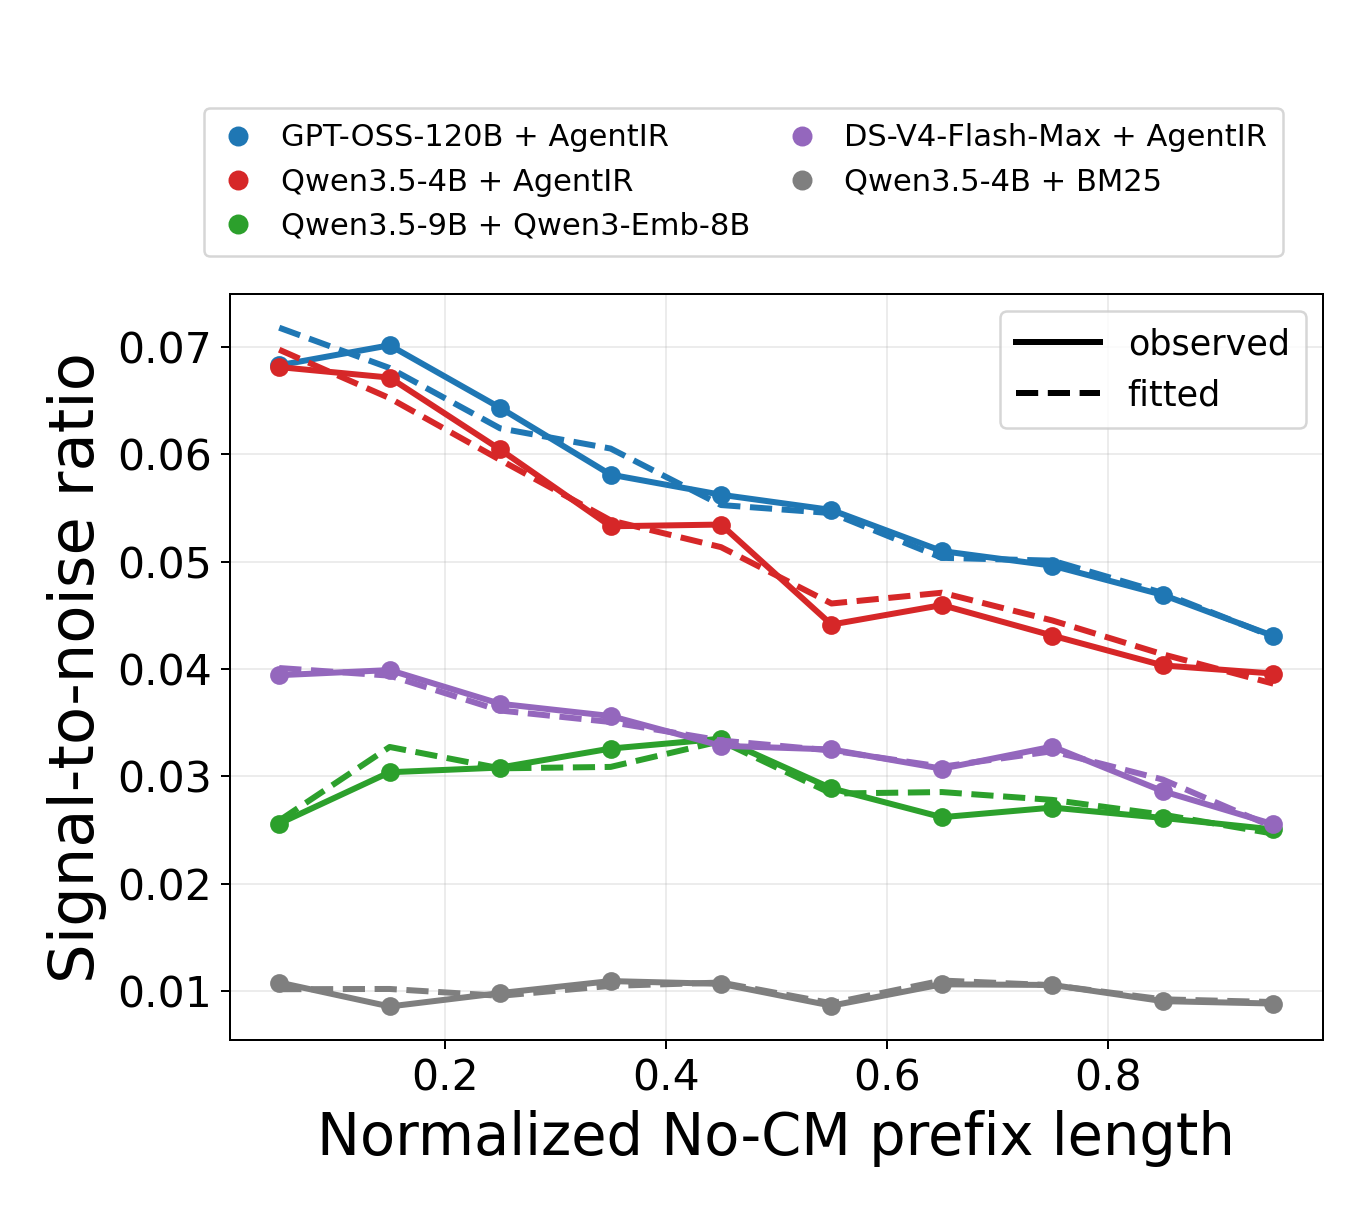
\includegraphics[width=\linewidth]{fig/trace_snr_curve_fit.png}
    \end{minipage}
    \hfill
    \raisebox{-0.5ex}{%
        \begin{minipage}[t]{0.73\textwidth}
            \centering
            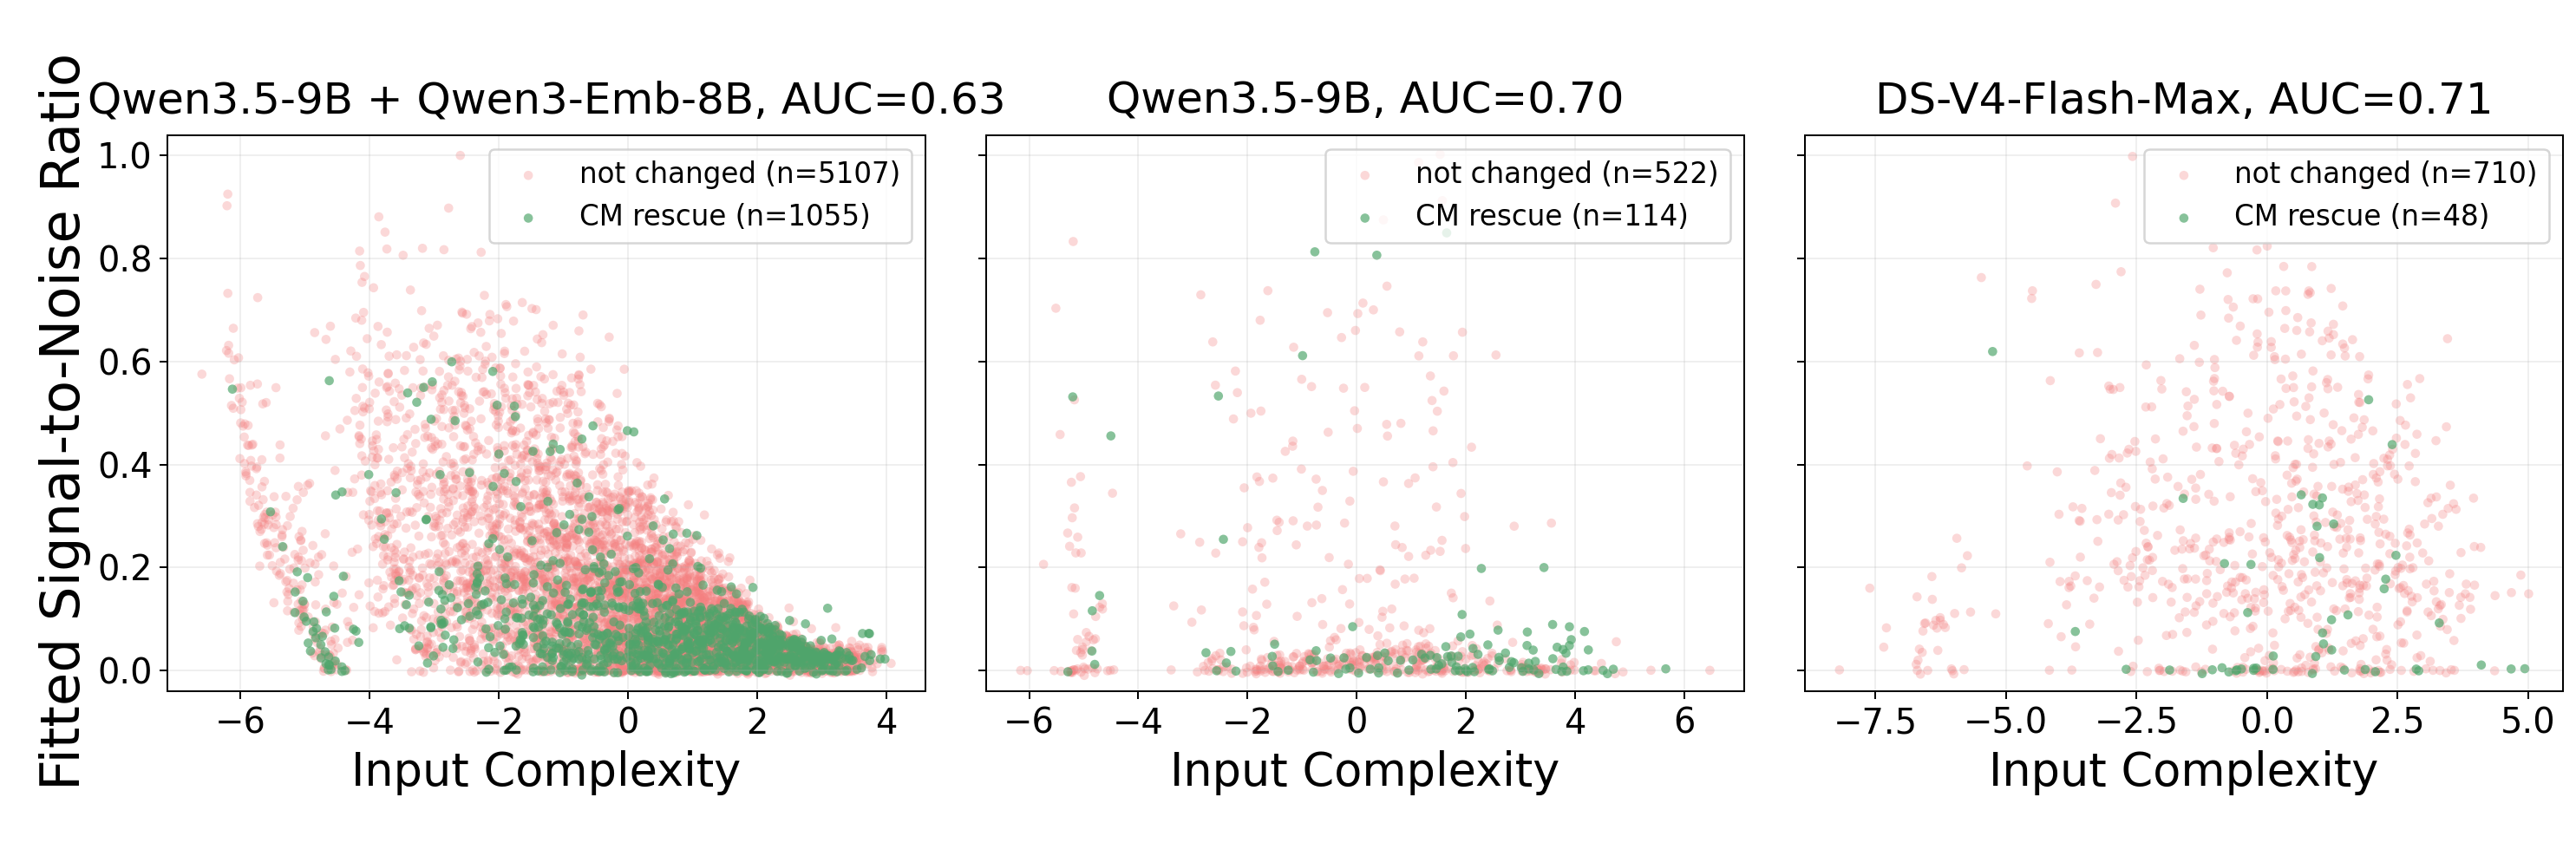
\includegraphics[width=\linewidth]{fig/snr_auc_dense.png}
        \end{minipage}%
    }
    % \hfill
    % \begin{minipage}[t]{0.46\textwidth}
    %     \centering
    %     \includegraphics[width=\linewidth]{fig/snr_auc_liveweb.png}
    % \end{minipage}
    \vspace{-2em}
    \caption{
    \textbf{Trace-SNR regression probe.}
  From left to right: BrowseComp-Plus observed/fitted gold-document signal;
  BrowseComp-Plus CM-rescue separability for Qwen3.5-9B+Qwen3-Emb-8B; xBench live-web proxy fitting-SNR for Qwen3.5-9B; and xBench live-web proxy fitting-SNR for DeepSeek-V4-Flash-Max.
  In scatter plots, green and red points denote the CM-rescued and the unchanged. A higher AUC score means a more separable prediction of whether CM rescues. xBench uses final-answer citation lines as a proxy because gold-document qrels are unavailable.
    }
    \vspace{-1em}
    \label{fig:probe}
\end{figure*}